\documentclass{article}

\usepackage{graphicx}

\title{Processing hydrolysis rate data in R}
\author{Drew Steen}

\usepackage{Sweave}
\begin{document}
%\Sconcordance{concordance:usingEnzalyzeInformal.tex:usingEnzalyzeInformal.Rnw:%
1 7 1 1 0 26 1}

\maketitle

\section*{Setup}
To get started, you'll need to install R (cran.r-project.org) and R's Integrated Development Environment (IDE), RStudio (rstudio.com)

Next, set up a folder on your hard drive for this project (say, \texttt{C:/documents/enzymeResearch}). Then, open up RStudio and make a new project: Choose \texttt{File, New Project, Existing Directory} and browse to your directory. 

Next, set up the following new folders in your project directory: \texttt{R}, \texttt{plots}, \texttt{data}, and \texttt{reports}. (Be sure to make the capitalization identical to mine so that our scripts will work on each others' systems.) Finally, save the file I've sent you, \texttt{lm\_stats.R}, to your \texttt{R} directory.

\section*{Prepare your data file}
Eventually, I plan to write functions that can deal with the plate reader output files directly. For now, open the .txt or Excel file from the plate reader, copy the section containing the raw data (usually starting at row 40 or so, be sure to include the row headers) into a new spreadsheet, and save it as a .csv file.

My original file looks like this:

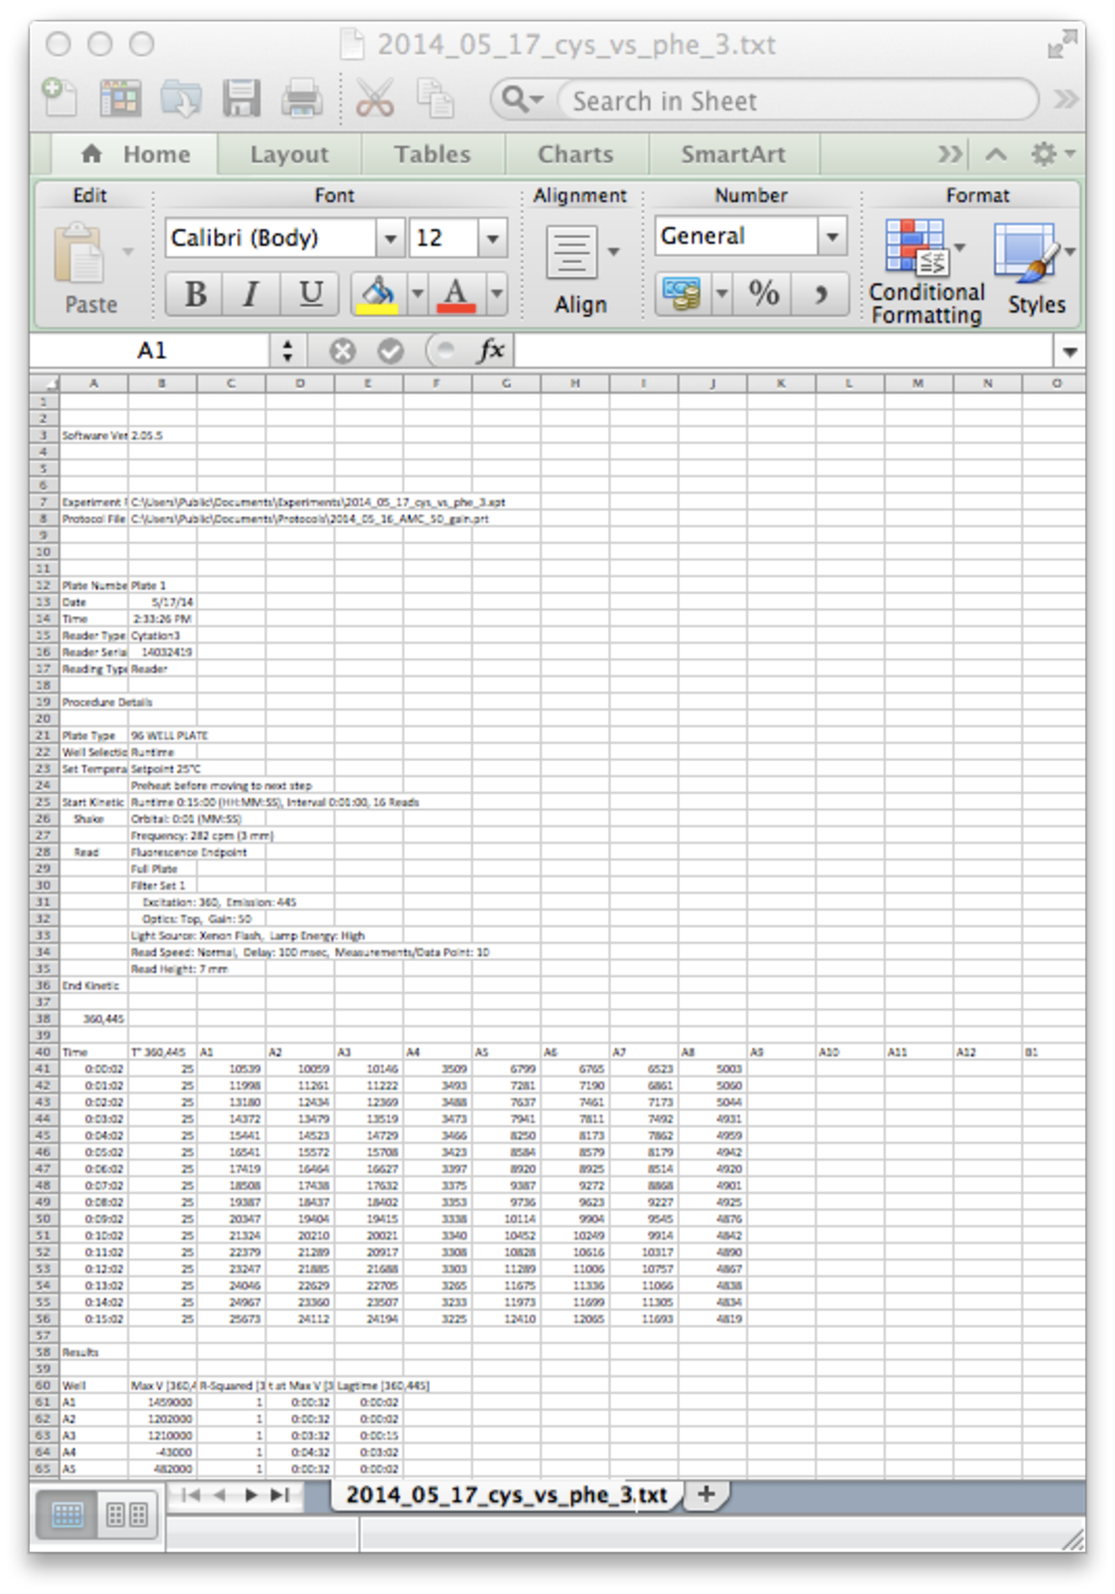
\includegraphics{raw_output.pdf}






\end{document}
